\documentclass[a4paper]{article}

\usepackage{times}
\usepackage{tikz}
\usepackage[margin=0cm]{geometry}
\usepackage{graphicx}
\usepackage{anyfontsize}
\usepackage{fancyhdr}
\usepackage{indentfirst}
\usepackage{amsmath}
\usepackage[spanish]{babel}
\usepackage[utf8]{inputenc}
\usepackage{titlesec}
\usepackage{enumitem}
\usepackage{caption}
\usepackage{booktabs}

\author{}
\date{}
\title{}

\begin{document}
\thispagestyle{empty}

\begin{tikzpicture}[remember picture, overlay]
    \pgftransformshift{\pgfpoint{0cm}{0cm}}
    \draw [line width=2pt](1cm,-1cm) -- (1cm,-27.7cm) -- (14cm, -27.7cm) -- (14cm, -1cm) -- (1cm, -1cm);
    \draw[line width=2pt] (15cm, -27.7cm) -- (19cm,-27.7cm) -- (19cm, -1cm) -- (15cm, -1cm) --  (15cm, -27.7cm);
    \node [line width=2pt] at (17cm, -3.5cm) {
\includegraphics[width=3cm]{../imagenes/utn.png}};
		\node [line width=2pt] at (7.5cm, -7.5cm) {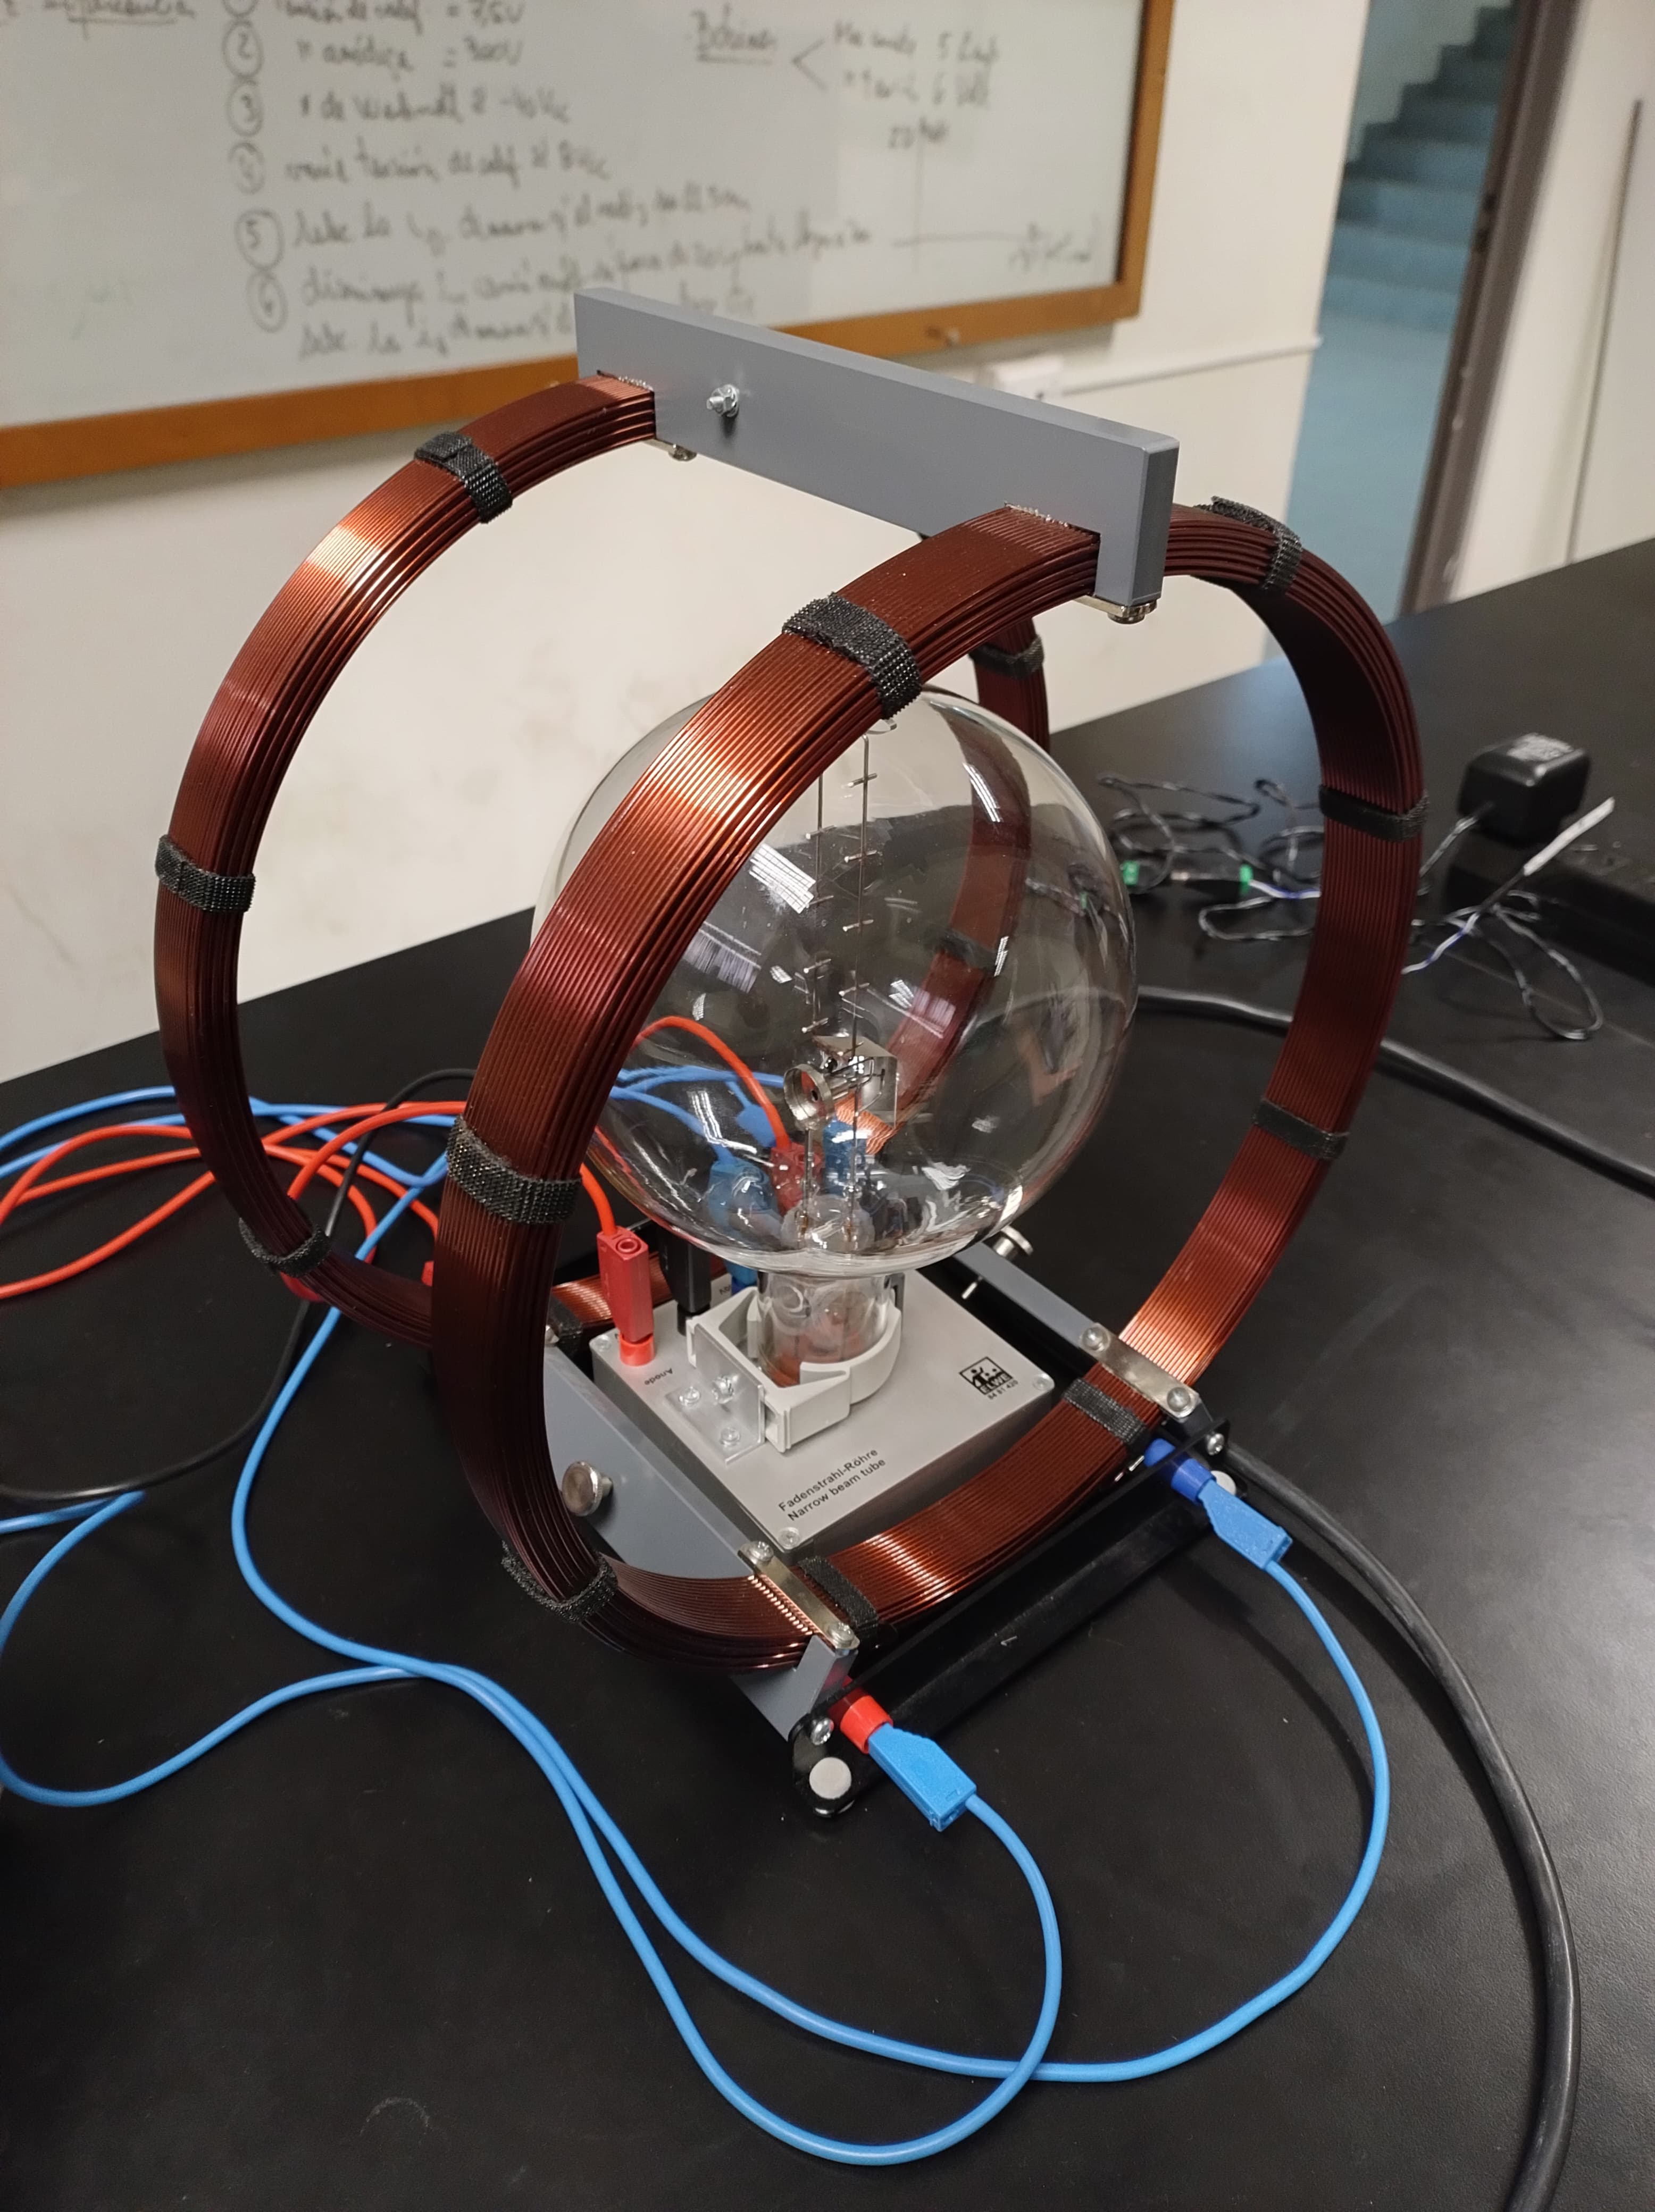
\includegraphics[width=6cm]{../imagenes/ampollaYBobinasHelmholtz.jpeg}};
    \node at (17cm, -7cm) {\scalebox{5}{\textbf{U}}};
    \node at (17cm, -9cm) {\scalebox{5}{\textbf{T}}};
    \node at (17cm, -11cm) {\scalebox{5}{\textbf{N}}};
    \node at (17cm, -14cm) {\scalebox{5}{\textbf{F}}};
    \node at (17cm, -16cm) {\scalebox{5}{\textbf{R}}};
    \node at (17cm, -18cm) {\scalebox{5}{\textbf{C}}};
    \node at (7.5cm, -13cm) {\scalebox{2.5}{\textbf{Carga específica}}};
    \node at (7.5cm, -14cm) {\scalebox{2.5} {\textbf{del electrón}}};

    \node at (7.5cm, -23cm) {
        \begin{minipage}[r]{12cm}
            \begin{itemize}
                \setlength{\itemsep}{-1em}
                \item \fontsize{12}{12}\selectfont \textbf{Autores:} \vspace {1mm} \fontsize{11}{12}\selectfont 
                    \begin{itemize}
                        \setlength{\itemsep}{-1em}
                        \item \hspace{2mm} Valentino Rao - Leg. 402308 \\
                        \item \hspace{2mm} Ignacio Ismael Perea - Leg. 406265 \\
                        \item \hspace{2mm} Manuel Leon Parfait - Leg. 406599 \\ 
                        \item \hspace{2mm} Gonzalo Filsinger - Leg. 400460 \\ 
                        \item \hspace{2mm} Agustín Coronel - Leg. 402010 \\
                        \item \hspace{2mm} Marcos Raúl Gatica - Leg. 402006 \\
                        \item \hspace{2mm} Santiago Pannunzio - Leg. 402350 \\
                    \end{itemize}

                \item \fontsize{12}{12}\selectfont \textbf{Curso:} 2R1. \\
                \item \fontsize{12}{12}\selectfont \textbf{Asignatura:} Física electrónica. \\
                \item \fontsize{12}{12}\selectfont \textbf{Institución:} Universidad Tecnológica Nacional - Facultad Regional de Córdoba \\

            \end{itemize}
        \end{minipage}};

\end{tikzpicture}

\renewcommand{\normalsize}{\fontsize{12}{18}\selectfont}
\newgeometry{margin=1.5cm}
\fancyhf{}
\renewcommand{\headrulewidth}{0pt}
\renewcommand{\footrulewidth}{0.4pt}
\fancyfoot[R]{Rao V. - Parfait M. - Filsinger G. - Perea I. - Pannunzio S - Coronel A - Gatica M. [\textbf{pág. \thepage}]}
\setlength{\footskip}{1cm} 
\newpage
\thispagestyle{empty}
\text{}

\titleformat{\section} {\fontsize{12}{12}\bfseries}{\thesection.}{0.5em}{\underline}

\newpage
\newpage

\thispagestyle{empty}
\setcounter{page}{0}
\tableofcontents

\newpage
\thispagestyle{fancy}
\twocolumn
\flushbottom
\section{INTRODUCCIÓN}

    \indent El objetivo de este informe es detallar la experiencia de laboratorio llevado a cabo para la medición de la carga específica del electrón.

    \subsection{Fundamentos teóricos}
    \indent La fuerza de Lorentz que afecta al electrón entre cátodo y ánodo, perpendicular al campo $\vec{B}$ generado por las bobinas de Helmholtz y perpendicular a la velocidad, es dada por:

    \begin{equation} 
        vec{F} = e (\vec{v} x \vec{B}) 
    \end{equation}

    \indent Esta fuerza provoca que el electrón adopte una trayectoria orbital, con un cierto radio. \\
    \indent Esto se puede relacionar con la expresión de una fuerza centrípeta que actúa sobre un cuerpo con masa que describe una circunferencia:

    \begin{equation}
        vec{F} = m {\frac {(\vec{v})^2}{r}}
    \end{equation}

    \indent Ambas expresiones de fuerza son iguales, por lo tanto se puede decir que:

    \begin{equation}
        e \vec{v} \vec{B} = m {\frac {(\vec{v})^2}{r}} \\ 
        e \vec{B} = m \frac {\vec{v}}{r}
    \end{equation}

    \indent Por otro lado, se sabe que la velocidad $\vec{v}$ depende de la tensión de aceleración $U$ del cañón de electrones:

    \begin{align}
        \vec{v} &= [2 (\frac {e}{m}) U]^{\frac{1}{2}} \tag*{} \\[10pt]
        \Rightarrow e \vec{B} &= \frac{m {\vec{v}}}{r} \tag*{} \\[10pt]
        e \vec{B} &= \frac{m[2 (\frac {e}{m}) U]^{\frac{1}{2}}}{r} \tag*{} \\[10pt]
        \frac{e}{m} &= \frac{[2 (\frac {e}{m}) U]^{\frac{1}{2}}}{r \vec{B}} \tag*{} \\[10pt]
        (\frac{e}{m})^{2} &= \frac{[2 (\frac {e}{m}) U]^{\frac{1}{2}}}{r \vec{B}} \tag*{} \\[10pt]
        \frac{e}{m} = \frac{2 U}{(r \vec{B})^2} \tag*{\textit{Carga específica del electrón}}
    \end{align}

    \indent Donde:
    \begin{itemize}
        \item e: carga del electrón.
        \item m: masa del electrón.
        \item U: energía de potencial.
        \item r: radio de la trayectoria circular del electrón.
        \item $\vec{B}$: valor del campo magnético.
    \end{itemize}

\newpage
\noindent
\thispagestyle{fancy}

\section{ELEMENTOS NECESARIOS}

        \subsection{Tubo de haz fino - rayos filiformes}

        \begin{figure}[h!]
            \centering
            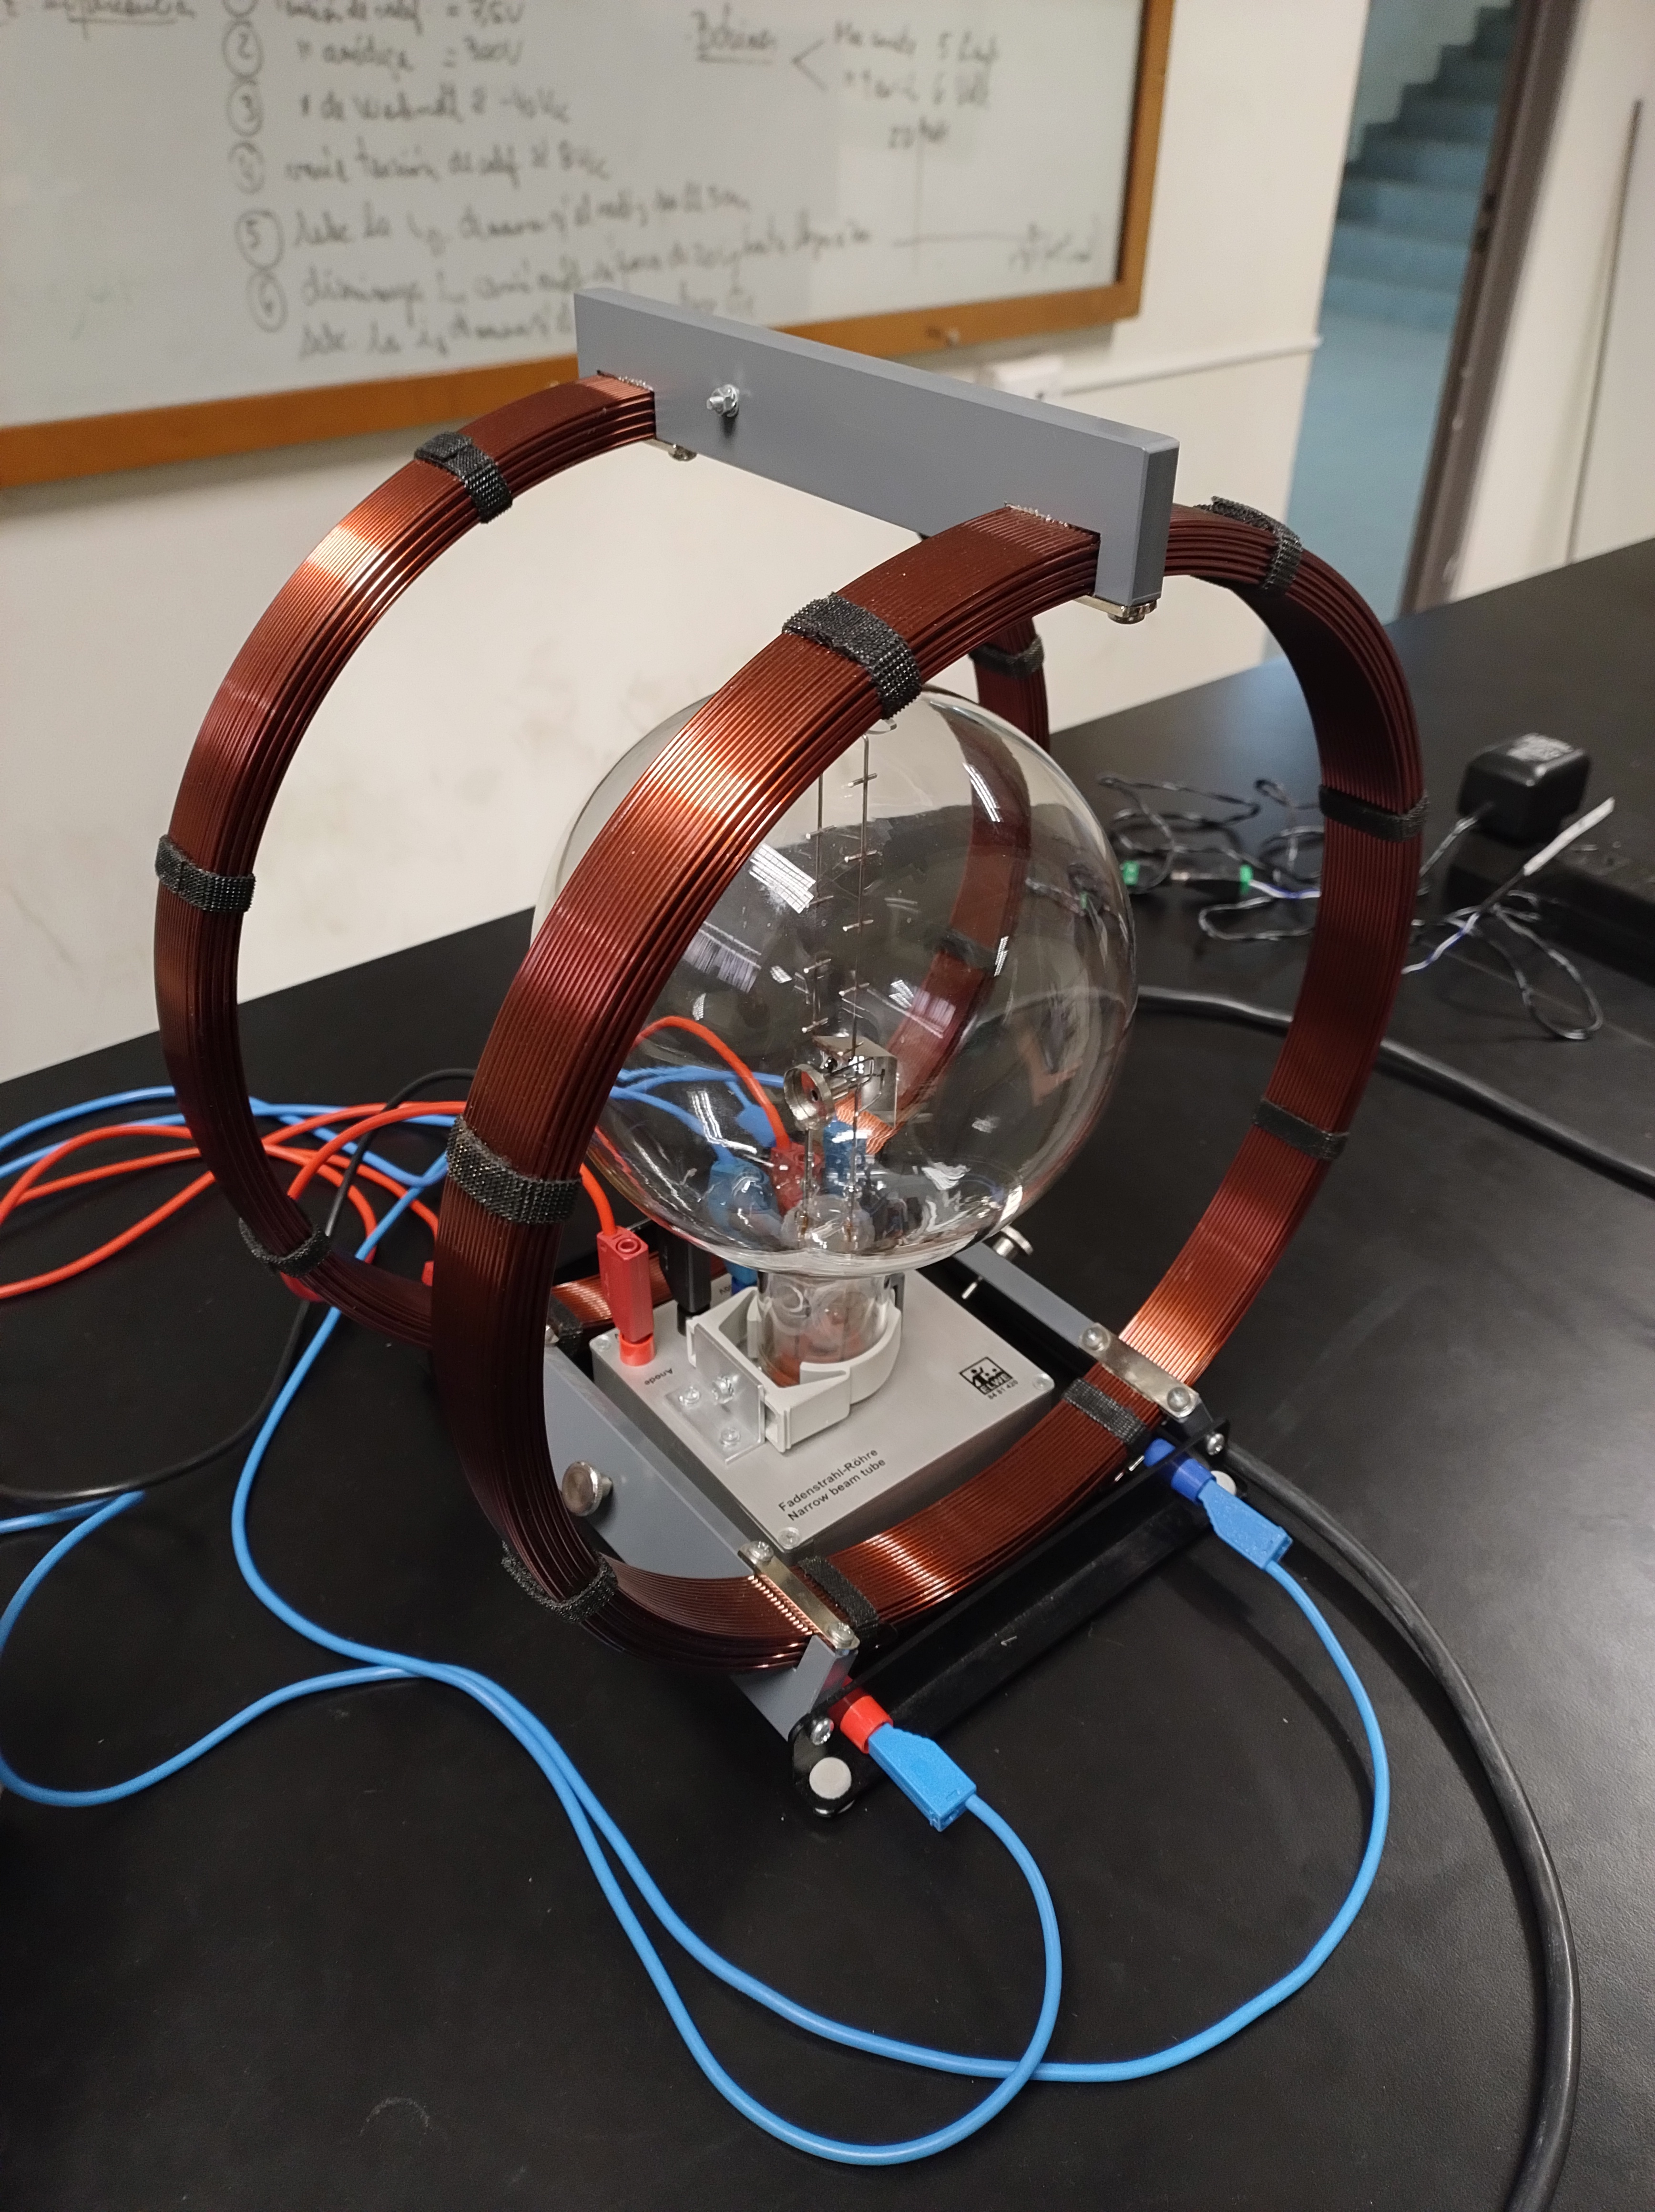
\includegraphics[width = 4.5cm] {../imagenes/tubodehazfino.jpg}
        \end{figure}

       \indent Es una ampolla rellena de neón a cierta presión ajustada precisamente en fábrica, con un cátodo y un ánodo que componen el cañón de electrones junto al cilindro de Wehnelt. Los átomos del gas son ionizados por los choques de los electrones que salen del cañón, el cual origina un rayo luminoso definido. \\
       \indent Se necesita entre 4 a 10 Vcc para calentarse y poder ver el efecto anteriormente mencionado. Además, se puede medir el diámetro de la circunferencia formada por el rayo de electrones usando una escala que trae la ampolla. La distancia entre las marcas de medición es de 20mm, y el diámetro de órbita de haz fino de radiación puede variar de entre 20 a 120mm. \\

    \subsection{Par de bobinas de Helmholtz}

        \begin{figure}[h!]
            \centering
            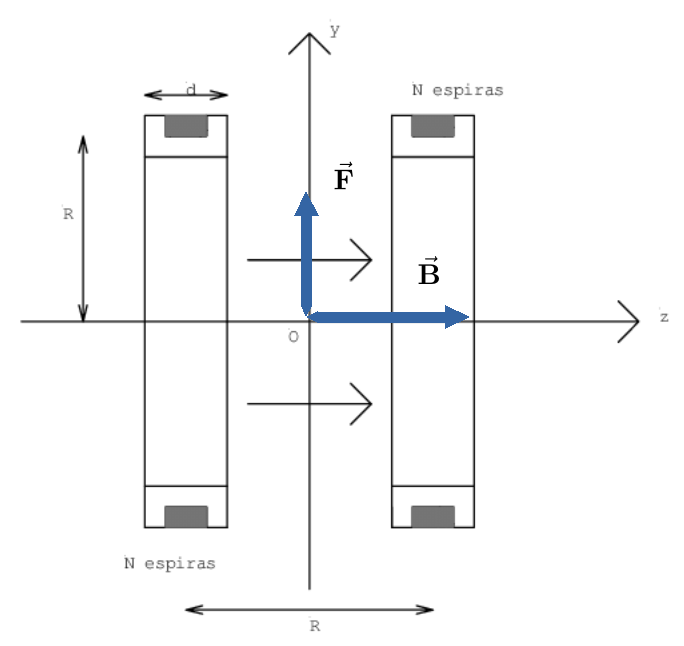
\includegraphics[width = 7.5cm] {../imagenes/dibujoBobinasHelmholtz.png}
        \end{figure}

        \begin{center}
            \textit{Vista lateral izquierda de las bobinas Helmholtz.}
        \end{center}

        \indent Estas bobinas producirán el campo magnético homogéneo entrante.

        \indent Lo destacable de este par de bobinas es que el número de espiras es de 124, funciona con una corriente máxima de 5A y una tensión máxima de 6V. \\

    \newpage
    \noindent
    \thispagestyle{fancy}

    \subsection{Fuente de alimentación para tubos}

        \begin{figure}[h!]
            \centering
            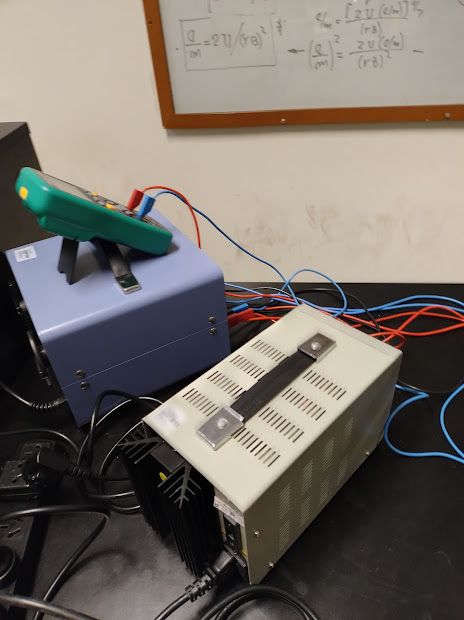
\includegraphics[width = 4.5cm] {../imagenes/fuentes.jpg}
        \end{figure}

        \indent Lo importante de la fuente usada es que:
        \begin{itemize}
            \item Puede variar la tensión de entre 0 a 300V (para el haz), y otro regulador de 0-50V (calentador).
            \item Permite regular la limitación de corriente entre 0-200mA.
            \item Clavijas de salida 0-300V, y de 0-50V.
            \item Masa común.
        \end{itemize}

    \subsection{Fuente de alimentación (bobinas)} 
    
        \indent Lo único importante de esta fuente es poder alimentar de manera estable las bobinas con sus valores de funcionamiento detallados en este índice.
       
    \subsection{Multímetro digital}

        \indent Lo importante de este instrumento es para verificar los voltajes de salida de las fuentes.

\section{MONTAJE}
    \renewcommand{\theenumi}{\roman{enumi}}

    \subsection{Esquema de conexiones}

        \begin{enumerate}
            \item Se colocó el tubo de rayos filiforme entre las bobinas de Helmholtz.

            \textbf{Conexión tubo de haz fino - fuente de alimentación}

            \item Conectar los clavijeros de masa entre sí (negros) de la salida de 50V y de la salida de 12V.
            \item Conectar el polo (+) de la salida de 300V con el ánodo (clavijeros rojos) y el polo negativo con el cátodo (clavijeros negros).
            \item Conectar el voltímetro a la salida de 300V para su medición.
            \item Conectar el polo negativo de la salida de 50V con el cilindro de Wehnelt (clavijeros azules).
            \item Conectar el polo positivo de la salida de 12V con la calefacción de cátodo (clavijeros verdes).
            \item Conectar el clavijero de puesta a tierra de la fuente de alimentación del tubo con el clavijero de tierra del tubo de haz fino de radiación.

\newpage
\noindent
\thispagestyle{fancy}

            \textbf{Conexión bobinas Helmholtz - fuente de alimentación}

            \item Se conectó las bobinas en serie a la fuente de alimentación con 12 Vcc.
        \end{enumerate}

        \begin{figure}[h!]
            \centering
            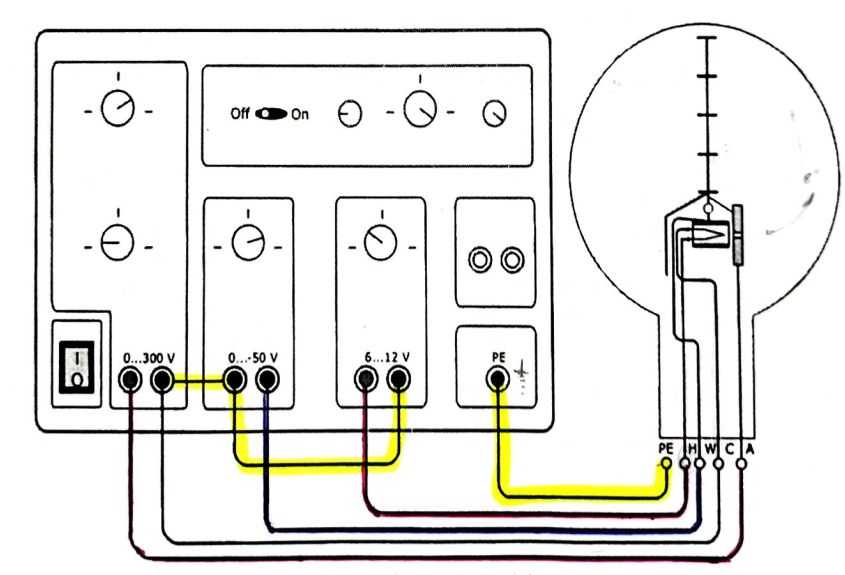
\includegraphics[width = 7cm] {../imagenes/esquemaConexionTuboDeHazFuenteAlim.png}
        \end{figure}

        \begin{center}
            \textit{Conexión Tubo de haz fino - Fuente de alimentación} \\
        \end{center}

        \begin{figure}[h!]
            \centering
            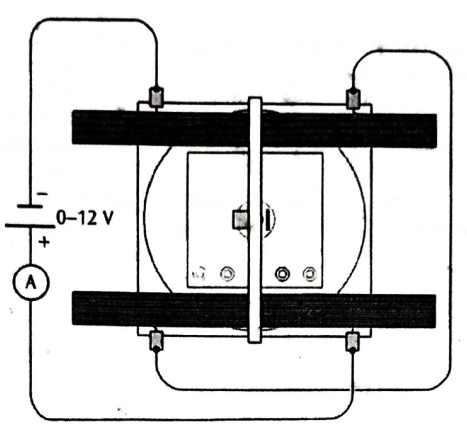
\includegraphics[width = 7cm] {../imagenes/esquemaConexionBobinasHelmholtzFuenteAlim.png}
        \end{figure}

        \begin{center}
            \textit{Conexión Bobinas de Helmholtz - Fuente de alimentación}
        \end{center}

    \subsection{Condiciones en el laboratorio}
        \begin{itemize}
            \item La experiencia se realizó a oscuras. 
            \item Se ajustó la tensión en el ánodo a 300V.
            \item Se reguló la tensión de Wehnelt para que se observe un haz de rayos delgado y definido.
            \item Se hizo variar la corriente de las bobinas ($I_H$) para ver cómo el haz se curva hacia arriba con el fin de medir los radios con la escala en la ampolla.
        \end{itemize}

\section{MEDICIONES}

    \renewcommand{\theenumi}{\roman{enumi}}
    \begin{enumerate}
        \item Se seleccionó la corriente de la bobina de manera que el radio de la órbita circular sea de 5cm y que el haz de electrones quede oculto por la marca de medición.
        \item Se disminuyó la tensión del ánodo de 20 en 20V hasta llegar a $\approx$ 160V. En cada caso, la $I_H$ empleada se ajustó para tener un radio constante.
        \item Se repitió el paso I y II pero con radios que iban disminuyendo cada 0,50cm hasta llegar a un radio de 2cm. \\
    \end{enumerate}
    
    \indent Para los calculos de $e \cdot m^{-1}$ y del campo magnético $B$ se utilizaron la siguientes fórmulas:

    \begin{equation}
        e\cdot m^{-1} = 2U\cdot (r\vec{B})^{-2}
    \end{equation}

    \begin{equation}
        B = K \cdot I_H
    \end{equation}

%    \newpage
%    \noindent
%    \thispagestyle{fancy}

    \indent Primero se calculó el promedio de $U$ y $I_H$ para cada radio, y luego se utilizó la fórmula (5) para calcular $e \cdot m^{-1}$ y la fórmula (6) para calcular $B$.
    \vspace{1mm}

    \begin{center}
        \begin{minipage}[c]{7.5cm}
            \centering
            \textbf{Radio: 5cm} 
            \vspace {2mm}
        \end{minipage}

        \begin{tabular}{ c c c }
            \toprule
            N \textdegree & $U$ (V) & $I_H$ (A)\\
            \midrule
            1 & 300 & 1.60 \\
            2 & 280 & 1.55 \\
            3 & 260.7 & 1.49 \\
            4 & 240.8 & 1.44 \\
            5 & 220.7 & 1.38 \\
            6 & 200.2 & 1.319 \\
            7 & 180.4 & 1.25 \\
            8 & 160.8 & 1.17 \\
            \bottomrule
        \end{tabular}
    \end{center}
    \vspace{1mm}

    \indent Los promedios de $U$ y $I_H$ para el radio de 5cm son de $230.15$V y $1.40$A respectivamente. Con estos valores calculamos $e \cdot m^{-1}$ y $B$, siendo estos valores de $1.644 \cdot 10^{11}$ C/kg y $1.06 \cdot 10^{-3}$ T respectivamente.
    \vspace{1cm}

    \begin{center}
        \begin{minipage}[c]{7.5cm}
            \centering
            \textbf{Radio: 4.5cm} 
            \vspace {2mm}
        \end{minipage}

        \begin{tabular}{ c c c }
            \toprule
            N \textdegree & $U$ (V) & $I_H$ (A)\\
            \midrule
            1 & 300 & 1.77 \\
            2 & 280.6 & 1.69 \\
            3 & 260 & 1.64 \\
            4 & 240.2 & 1.58 \\
            5 & 220.2 & 1.51 \\
            6 & 200 & 1.44 \\
            7 & 180 & 1.37 \\
            8 & 160.2 & 1.27 \\
            \bottomrule
        \end{tabular} 
    \end{center}
    \vspace{1mm}

    \indent Los promedios de $U$ y $I_H$ para el radio de 4.5cm son de $230.15$V y $1.533$A respectivamente. Con estos valores calculamos $e \cdot m^{-1}$ y $B$, siendo estos valores de $1.636 \cdot 10^{11}$ C/kg y $1.16 \cdot 10^{-3}$ T respectivamente.
    \vspace{1cm}

    \begin{center}
        \begin{minipage}[c]{7.5cm}
            \centering
            \textbf{Radio: 4cm} 
            \vspace {2mm}
        \end{minipage}

        \begin{tabular}{ c c c }
            \toprule
            N \textdegree & $U$ (V) & $I_H$ (A)\\
            \midrule
            1 & 300.5 & 1.979 \\
            2 & 280.3 & 1.92 \\
            3 & 260.6 & 1.85 \\
            4 & 240.1 & 1.769 \\
            5 & 220.4 & 1.709 \\
            6 & 200.1 & 1.61 \\
            7 & 180.6 & 1.529 \\
            8 & 160.1 & 1.44 \\
            \bottomrule
        \end{tabular}
    \end{center}
    \vspace{1mm}

    \indent Los promedios de $U$ y $I_H$ para el radio de 4cm son de $230.34$V y $1.725$A respectivamente. Con estos valores calculamos $e \cdot m^{-1}$ y $B$, siendo estos valores de $1.634 \cdot 10^{11}$ C/kg y $1.31 \cdot 10^{-3}$ T respectivamente.
    \vspace{1cm}

    % \newpage
    % \noindent
   \thispagestyle{fancy}

    \begin{center}
        \begin{minipage}[c]{7.5cm}
            \centering
            \textbf{Radio: 3.5cm} 
            \vspace {2mm}
        \end{minipage}

        \begin{tabular}{ c c c }
            \toprule
            N \textdegree & $U$ (V) & $I_H$ (A)\\
            \midrule
            1 & 300.4 & 2.25 \\
            2 & 280.5 & 2.179 \\
            3 & 260 & 2.14 \\
            4 & 240.3 & 2.03 \\
            5 & 220.2 & 1.969 \\
            6 & 200.1 & 1.859 \\
            7 & 180.1 & 1.77 \\
            8 & 160.3 & 1.65 \\
            \bottomrule
        \end{tabular}
    \end{center}
    \vspace{1mm}

    \indent Los promedios de $U$ y $I_H$ para el radio de 3.5cm son de $230.24$V y $1.98$A respectivamente. Con estos valores calculamos $e \cdot m^{-1}$ y $B$, siendo estos valores de $1.688 \cdot 10^{11}$ C/kg y $1.5 \cdot 10^{-3}$ T respectivamente.
    \vspace{1cm}

    \begin{center}
        \begin{minipage}[c]{7.5cm}
            \centering
            \textbf{Radio: 3cm} 
            \vspace {2mm}
        \end{minipage}

        \begin{tabular}{ c c c }
            \toprule
            N \textdegree  &  $U$ (V)  &  $I_H$ (A) \\
            \midrule
            1 & 300.3 & 2.65 \\
            2 & 280.2 & 2.56 \\
            3 & 260 & 2.48 \\
            4 & 240.5 & 2.38 \\
            5 & 220.1 & 2.27 \\
            6 & 200.2 & 2.18 \\
            7 & 180 & 2.05 \\
            8 & 160 & 1.95 \\
            \bottomrule
        \end{tabular}
    \end{center}
    \vspace{1mm}

    \indent Los promedios de $U$ y $I_H$ para el radio de 3cm son de $230.24$V y $2.315$A respectivamente. Con estos valores calculamos $e \cdot m^{-1}$ y $B$, siendo estos valores de $1.665 \cdot 10^{11}$ C/kg y $1.75 \cdot 10^{-3}$ T respectivamente.
    \vspace{1cm}

    \begin{center}
        \begin{minipage}[c]{7.5cm}
            \centering
            \textbf{Radio: 2.5cm} 
            \vspace {2mm}
        \end{minipage}

        \begin{tabular}{ c c c }
            \toprule
            N \textdegree & $U$ (V) & $I_H$ (A)\\
            \midrule
            1 & 300 & 3.26 \\
            2 & 280.6 & 3.13 \\
            3 & 260.2 & 3.03 \\
            4 & 240.5 & 2.87 \\
            5 & 220.2 & 2.76 \\
            6 & 200.2 & 2.56 \\
            7 & 180.1 & 2.42 \\
            8 & 160.3 & 2.33 \\
            \bottomrule
        \end{tabular}
    \end{center}
    \vspace{1mm}

    \indent Los promedios de $U$ y $I_H$ para el radio de 2.5cm son de $230.26$V y $2.795$A respectivamente. Con estos valores calculamos $e \cdot m^{-1}$ y $B$, siendo estos valores de $1.440 \cdot 10^{11}$ C/kg y $2.12 \cdot 10^{-3}$ T respectivamente.
    \vspace{1cm}

    \newpage
    \noindent
    \thispagestyle{fancy}

    \begin{center}
        \begin{minipage}[c]{7.5cm}
            \centering
            \textbf{Radio: 2cm} 
            \vspace {2mm}
        \end{minipage}

        \begin{tabular}{ c c c }
            \toprule
            N \textdegree & $U$ (V) & $I_H$ (A)\\
            \midrule
            1 & 300.5 & 4.01 \\
            2 & 280.2 & 3.88 \\
            3 & 260 & 3.73 \\
            4 & 240.1 & 3.60 \\
            5 & 220.2 & 3.45 \\
            6 & 200.5 & 3.31 \\
            7 & 180.2 & 3.13 \\
            8 & 160.3 & 2.92 \\
            \bottomrule
        \end{tabular}
    \end{center}
    \vspace{1mm}

    \indent Los promedios de $U$ y $I_H$ para el radio de 2cm son de $230.25$V y $3.5$A respectivamente. Con estos valores calculamos $e \cdot m^{-1}$ y $B$, siendo estos valores de $1.637 \cdot 10^{11}$ C/kg y $2.65 \cdot 10^{-3}$ T respectivamente.
    \vspace{1cm}

    \begin{center}
        \begin{minipage}[c]{7.5cm}
            \centering
            \textbf{Tabla de promedios}
            \vspace {2mm}
        \end{minipage}

        \begin{tabular}{ c c c c c }
            \toprule
            R (cm) & $U$ (V) & $I_H$ (A) & $e \cdot m^{-1}$ (C/kg) & $B$ (T)\\
            \midrule
            5 & 230.15 & 1.40 & $1.644 \cdot 10^{11}$ & $1.06 \cdot 10^{-3}$ \\
            4.5 & 230.15 & 1.533 & $1.636 \cdot 10^{11}$ & $1.16 \cdot 10^{-3}$ \\
            4 & 230.34 & 1.725 & $1.634 \cdot 10^{11}$ & $1.31 \cdot 10^{-3}$ \\
            3.5 & 230.24 & 1.98 & $1.688 \cdot 10^{11}$ & $1.5 \cdot 10^{-3}$ \\
            3 & 230.24 & 2.315 & $1.665 \cdot 10^{11}$ & $1.75 \cdot 10^{-3}$ \\
            2.5 & 230.26 & 2.795 & $1.440 \cdot 10^{11}$ & $2.12 \cdot 10^{-3}$ \\
            2 & 230.25 & 3.5 & $1.637 \cdot 10^{11}$ & $2.65 \cdot 10^{-3}$ \\
            \bottomrule
        \end{tabular}
    \end{center}

    \indent Si sabemos que $e \cdot m^{-1}$ es igual a $2U \cdot (r \cdot B)^{-2}$, si despejamos $2U$ obtenemos que $2U = (r \cdot B)^2 \cdot (e \cdot m^{-1}) $ Por lo tanto, si graficamos $2U$ en función de $(r \cdot B)^2$, la pendiente de la recta será $e \cdot m^{-1}$, sabemos que $r$ es constante y que $B = K \cdot I_H$, donde $K$ la calculamos de la siguiente manera:\\

    \begin{equation}
        K = (\frac{4}{5})^{\frac{3}{2}} \cdot mu_{0} \cdot \frac{U}{R}
    \end{equation}
    
    \begin{equation}
        K = 7,584 \cdot 10^{-4} \frac{T \cdot m}{A} 
    \end{equation}

    \indent Entonces nos queda que $B = 7,584 \cdot 10^{-4} \cdot I_H$ y que la función para calcular $2U$ es:

    \begin{equation}
        2U = (r \cdot 7,584 \cdot 10^{-4} \cdot I_H)^2 \cdot (e \cdot m^{-1})
    \end{equation}

    \indent Sabemos los promedios de $U$ y $I_H$ para cada radio, y ya calculamos cuanto valen $e \cdot m^{-1}$ y $B$ para cada radio, con estos datos podemos graficar $2U$ en función de $(r \cdot B)^2$ y obtener la pendiente de la recta que será $e \cdot m^{-1}$.



    \indent Ahora podemos aplicar la fórmula (8) para calcular $2U$ y graficarla en función de $(r \cdot B)^2$. 
   
    \newpage
    \noindent
    \thispagestyle{fancy}
    
    \subsection{Gráficos}
    
    \begin{figure}[h!]
        \centering
        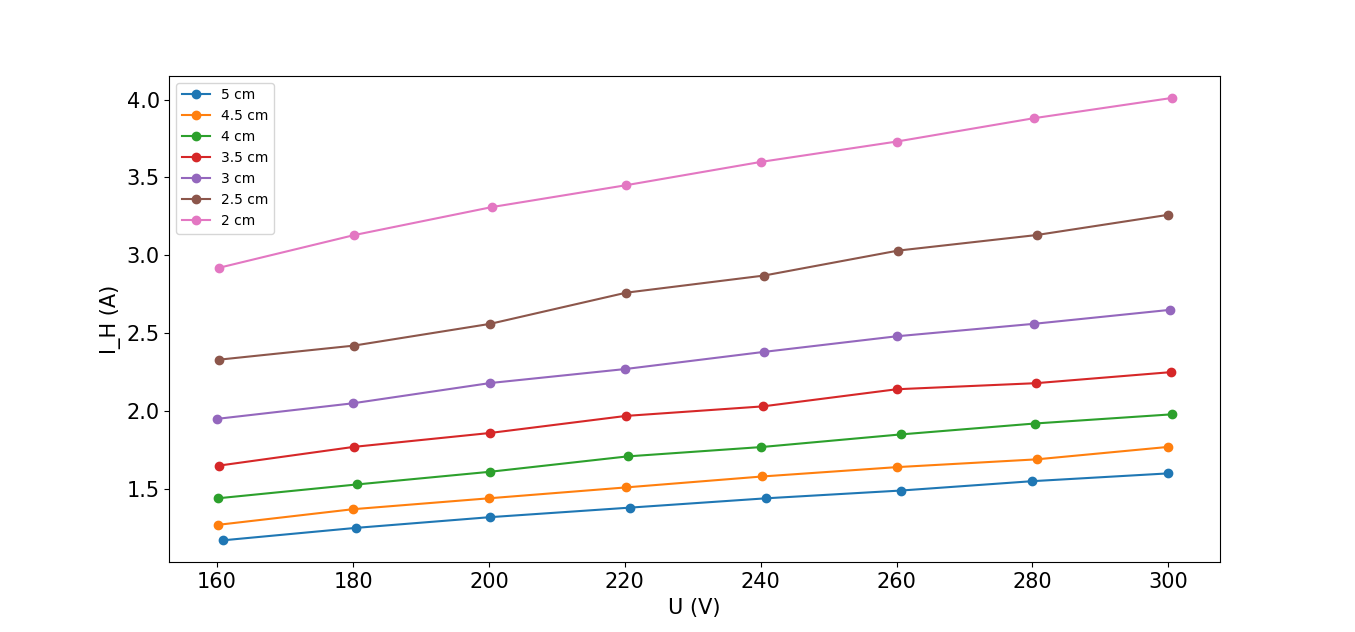
\includegraphics[width = 10.5cm] {../imagenes/graficoI_HyU.png}
        % \caption{Gráfico de $I_H$ en función de $U$ (Todos los radios)}
    \end{figure}

    \begin{center}
        \textbf{Gráfico de $I_H$ en función de $U$ (Todos los radios)}
    \end{center}

    \indent En el gráfico podemos observar que, a medida que disminuye el radio de la órbita, la corriente de las bobinas aumenta. Esto se debe a que, al disminuir el radio, la fuerza de Lorentz que actúa sobre los electrones es mayor, lo que requiere un campo magnético más intenso para mantener la órbita circular. Por lo tanto, la corriente en las bobinas de Helmholtz debe aumentar para generar un campo magnético más fuerte y contrarrestar la fuerza de Lorentz. Esto es consistente con nuestra suposición teórica de que la corriente en las bobinas es proporcional al campo magnético y, por lo tanto, a la fuerza de Lorentz, logrando poder medir la carga específica del electrón.

    \begin{figure}[h!]
        \centering
        \vspace{-2mm}
        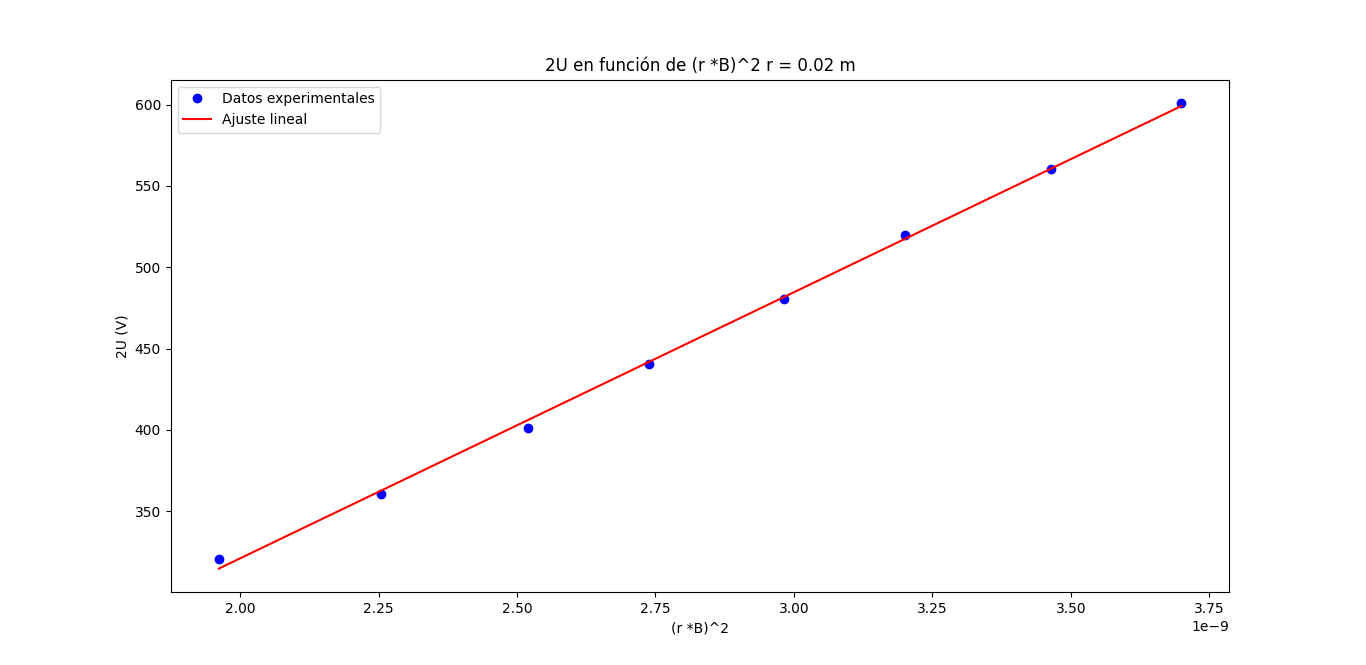
\includegraphics[width = 10cm] {../imagenes/radio2.png}
        % \textbf{$Pendiente: 1.637 \cdot 10^{11} C/kg$}
        % \caption{Gráfico de $2U$ en función de $(r \cdot B)^2$ con radio 2cm}
        \vspace{-5mm}
    \end{figure}

    \begin{center}
        \textbf{$Pendiente: 1.637 \cdot 10^{11} C/kg$} \\
        \textbf{Gráfico de $2U$ en función de $(r \cdot B)^2$ con radio 2cm} \\
    \end{center}

    \begin{figure}[h!]
        \centering
        \vspace{-2mm}
        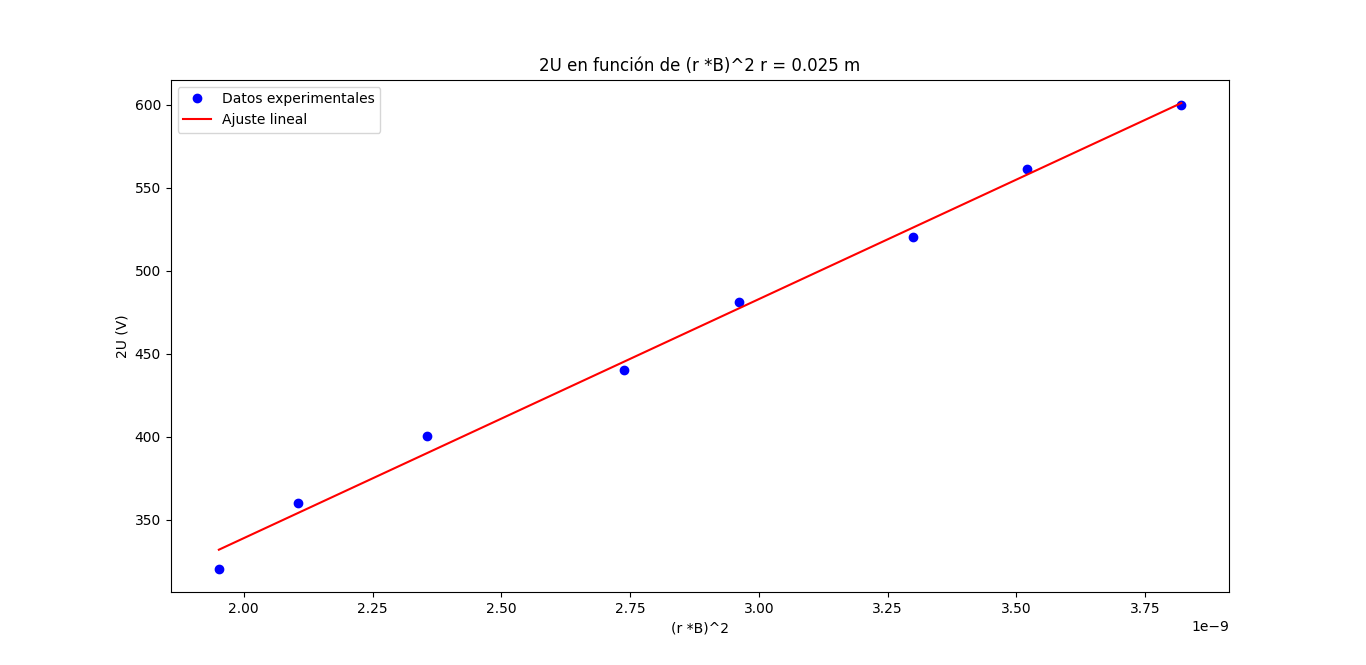
\includegraphics[width = 8cm] {../imagenes/radio2,5.png}
        % \textbf{$Pendiente: 1.440 \cdot 10^{11} C/kg$}
        % \caption{Gráfico de $2U$ en función de $(r \cdot B)^2$ con radio 2,5cm}
        \vspace{-5mm}
    \end{figure}

    \begin{center}
        \textbf{$Pendiente: 1.440 \cdot 10^{11} C/kg$} \\
        \textbf{Gráfico de $2U$ en función de $(r \cdot B)^2$ con radio 2,5cm} \\
    \end{center}

    \newpage
    \noindent
    \thispagestyle{fancy}

    \begin{figure}[h!]
        \centering
        \vspace{-2mm}
        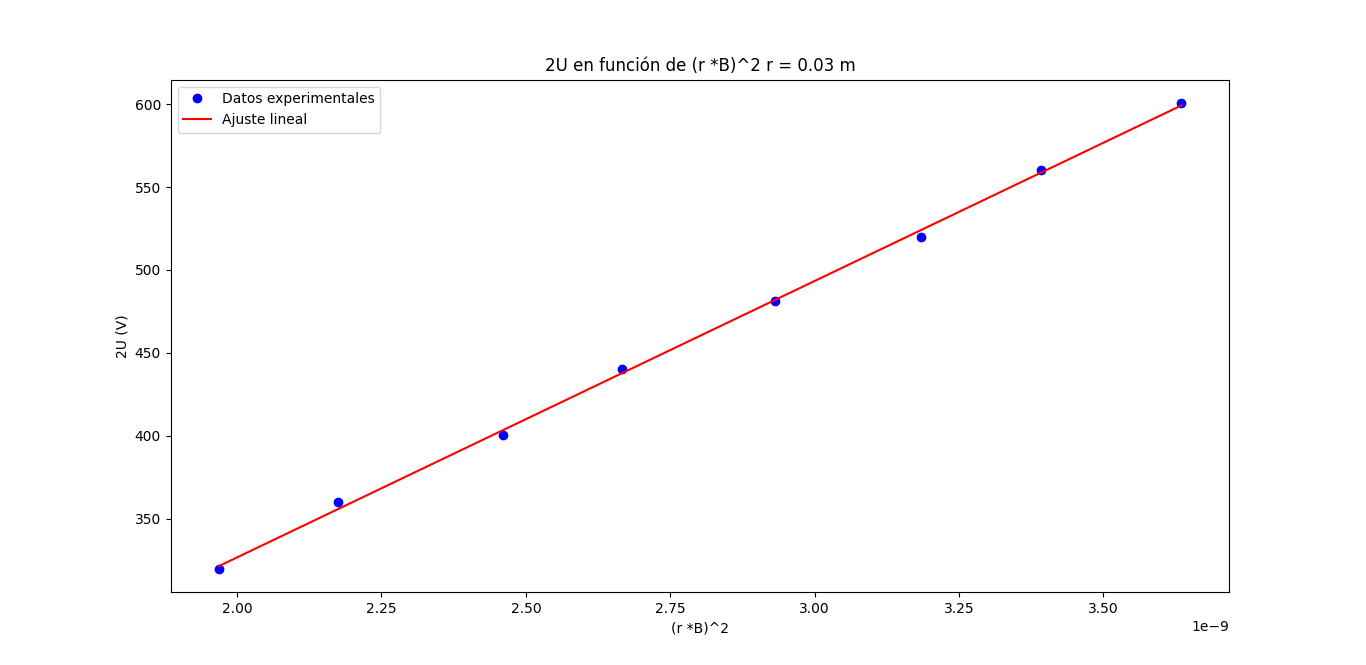
\includegraphics[width = 8cm] {../imagenes/radio3.png}
        % \textbf{$Pendiente: 1.665 \cdot 10^{11} C/kg$}
        % \caption{Gráfico de $2U$ en función de $(r \cdot B)^2$ con radio 3cm}
        \vspace{-5mm}
    \end{figure}

    \begin{center}
        \textbf{$Pendiente: 1.665 \cdot 10^{11} C/kg$} \\
        \textbf{Gráfico de $2U$ en función de $(r \cdot B)^2$ con radio 3cm} \\
    \end{center}

    \begin{figure}[h!]
        \centering
        \vspace{-2mm}
        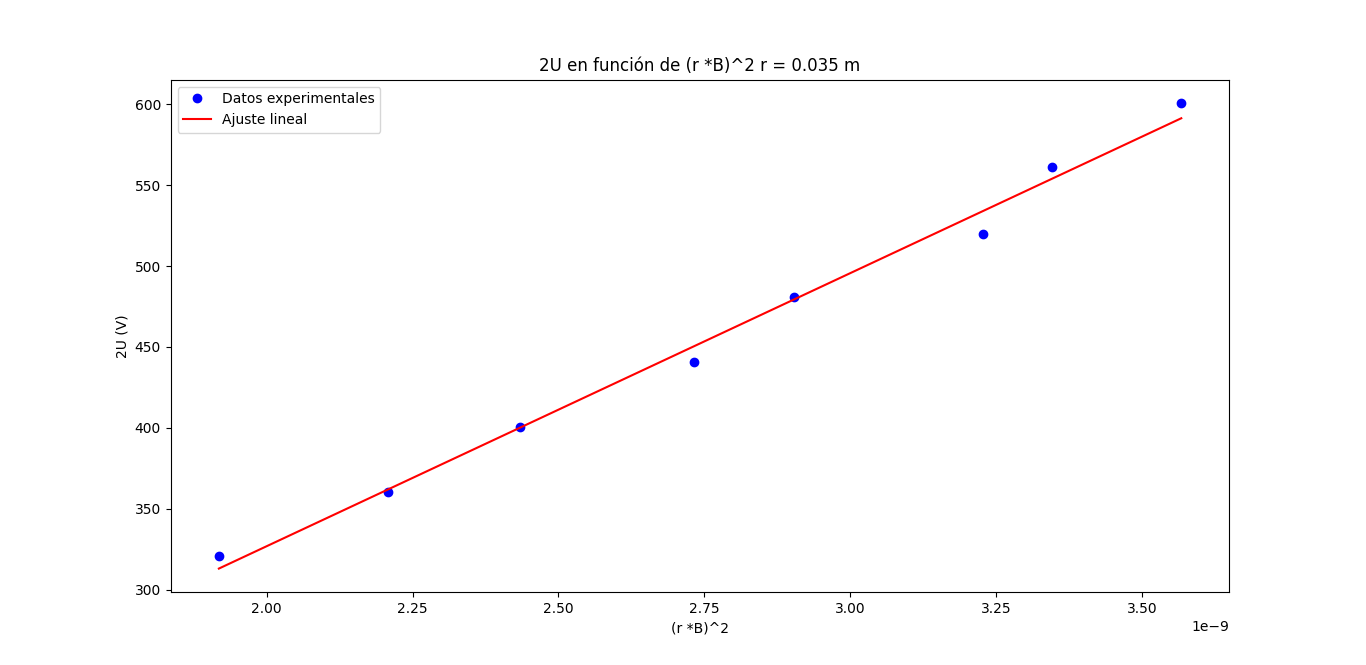
\includegraphics[width = 8cm] {../imagenes/radio3,5.png}
        % \textbf{$Pendiente: 1.688 \cdot 10^{11} C/kg$}
        % \caption{Gráfico de $2U$ en función de $(r \cdot B)^2$ con radio 3,5cm}
        \vspace{-5mm}
    \end{figure}

    \begin{center}
        \textbf{$Pendiente: 1.688 \cdot 10^{11} C/kg$} \\
        \textbf{Gráfico de $2U$ en función de $(r \cdot B)^2$ con radio 3,5cm} \\
    \end{center}

    \begin{figure}[h!]
        \centering
        \vspace{-2mm}
        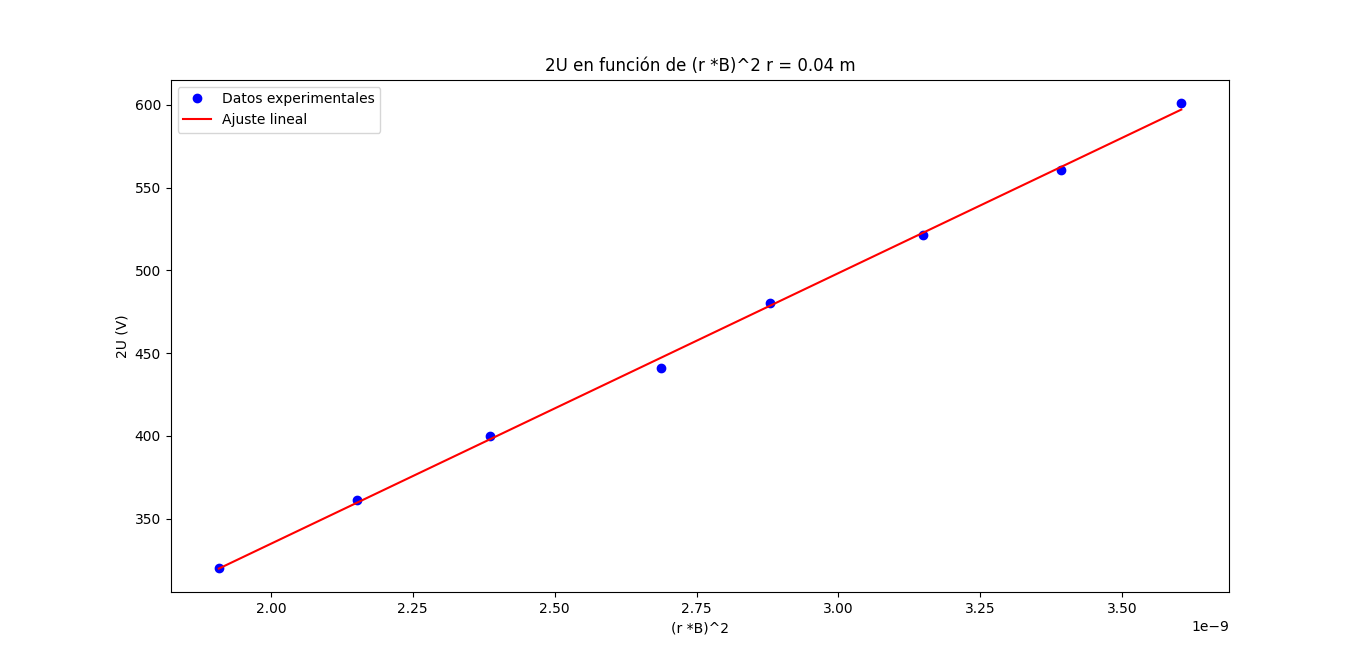
\includegraphics[width = 8cm] {../imagenes/radio4.png}
        % \textbf{$Pendiente: 1.634 \cdot 10^{11} C/kg$}
        % \caption{Gráfico de $2U$ en función de $(r \cdot B)^2$ con radio 4cm}
        \vspace{-5mm}
    \end{figure}

    \begin{center}
        \textbf{$Pendiente: 1.634 \cdot 10^{11} C/kg$} \\
        \textbf{Gráfico de $2U$ en función de $(r \cdot B)^2$ con radio 4cm} \\
    \end{center}

    \begin{figure}[h!]
        \vspace{-2mm}
        \centering
        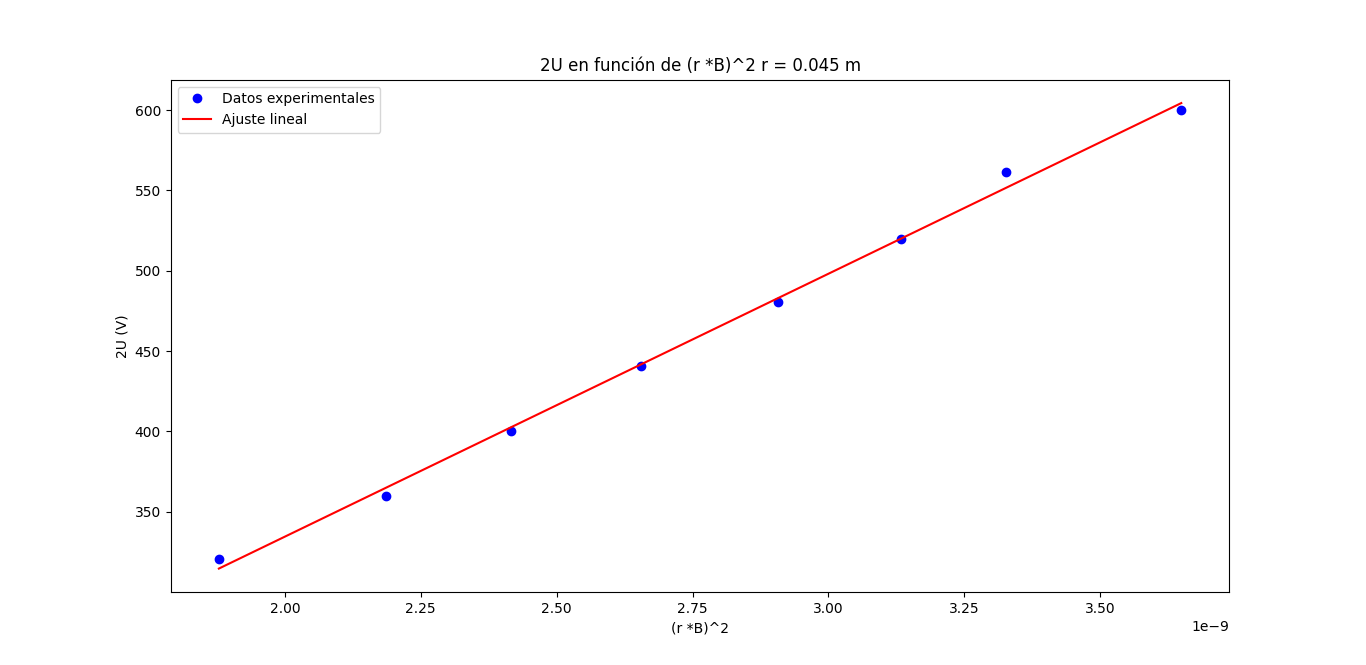
\includegraphics[width = 8cm] {../imagenes/radio4,5.png}
        % \textbf{$Pendiente: 1.636 \cdot 10^{11} C/kg$}
        % \caption{Gráfico de $2U$ en función de $(r \cdot B)^2$ con radio 4,5cm}
        \vspace{-5mm}
    \end{figure}

    \begin{center}
        \textbf{$Pendiente: 1.636 \cdot 10^{11} C/kg$} \\
        \textbf{Gráfico de $2U$ en función de $(r \cdot B)^2$ con radio 4,5cm} \\
    \end{center}

    \begin{figure}[h!]
        \vspace{-2mm}
        \centering
        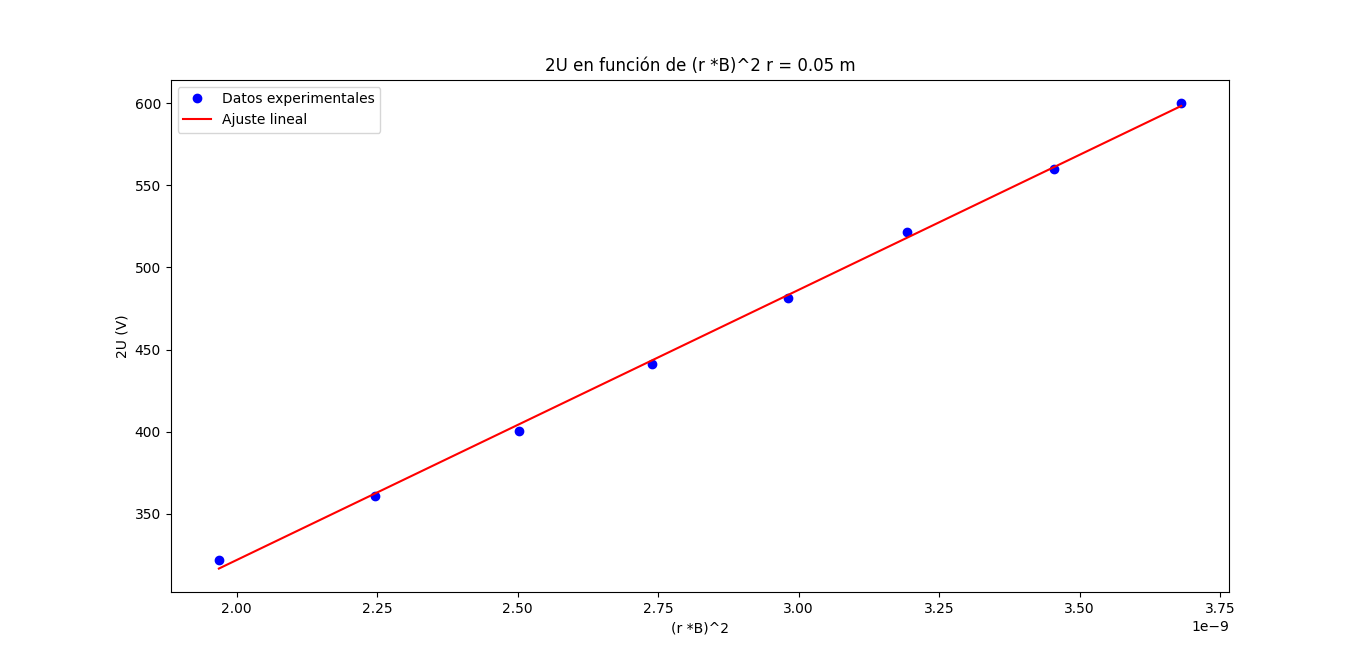
\includegraphics[width = 8cm] {../imagenes/radio5.png}
        % \textbf{$Pendiente: 1.644 \cdot 10^{11} C/kg$}
        % \caption{Gráfico de $2U$ en función de $(r \cdot B)^2$ con radio 5cm}
        \vspace{-5mm}
    \end{figure}

    \begin{center}
        \textbf{$Pendiente: 1.644 \cdot 10^{11} C/kg$} \\
        \textbf{Gráfico de $2U$ en función de $(r \cdot B)^2$ con radio 5cm} \\
    \end{center}

    \newpage
    \noindent
    \thispagestyle{fancy}

    \indent Calculando el promedio de las pendientes $e \cdot m^{-1}$ obtenemos un valor de 1.620 $\cdot 10^{11}$ C/kg, el cual es un valor muy cercano al valor teórico de 1.76 $\cdot 10^{11}$ C/kg, siendo nuestro error de un 8.5\%.


\section{CONCLUSIONES}

    \indent A través de este experimento, logramos estimar la relación carga-masa del electrón $e \cdot m^{-1}$ utilizando un tubo de vacío y bobinas de Helmholtz para generar un campo magnético uniforme. Observando el movimiento circular de los electrones bajo la influencia del campo magnético y aplicando principios de la física clásica, como la fuerza de Lorentz, la conservación de la energía y el movimiento circular uniforme, pudimos derivar y calcular este valor fundamental en la física.

    Los resultados obtenidos estuvieron dentro de un margen razonable respecto al valor teórico de $e \cdot m^{-1}$, lo cual sugiere que el montaje experimental y los métodos de medición fueron adecuados. Sin embargo, también se evidenciaron algunas fuentes de error, como posibles imprecisiones en la medición del radio de la trayectoria de los electrones, fluctuaciones en la corriente de las bobinas de Helmholtz y variaciones en el voltaje de aceleración. Estas limitaciones pudieron haber causado desviaciones menores respecto al valor teórico, destacando la importancia de la calibración y la precisión en experimentos de física.

    Este experimento no solo permitió corroborar el valor conocido de la carga específica del electrón, sino que también ofreció una oportunidad de profundizar en el estudio de partículas subatómicas y en la relación entre los campos magnéticos y eléctricos y las partículas cargadas. De este modo, comprendimos cómo los principios clásicos son aplicables incluso a partículas tan pequeñas como los electrones, un descubrimiento que fue clave para el desarrollo de la teoría atómica y que sigue siendo relevante hoy en día en la física moderna.

    En conclusión, el experimento nos permitió valorar la importancia de la metodología y precisión en mediciones experimentales, además de brindar una comprensión profunda de la naturaleza de los electrones y su interacción con campos electromagnéticos. A pesar de los desafíos y limitaciones, logramos cumplir nuestro objetivo de calcular $e \cdot m^{-1}$ y obtener un resultado consistente con los principios teóricos.

\end{document}
